% !Mode:: "TeX:UTF-8"

\chapter{绪论}[Introduction]

\section{课题背景及研究的目的和意义}[Background]
知识图谱作为人工智能的重要基石,近些年得到了不断的发展和应用。特别是搜索引擎开始
利用知识图谱来改进搜索的质量,加快搜索的速度,并且实现语义搜索和推理。

知识图谱是由语义表示的网络,它能够帮助使用者搜索知识网络中的所有知识。知识网络是
由许多个实体,属性和属性值构成的。有全局唯一的标识符URI来表示一个实体,属性是用
来描述实体的内在特性或实体之间的关联关系。W3C提出了一种资源描述框架RDF\cite{rdf}
来表示知识图谱网络,一条知识表示为一个SPO三元组(Subject,Predicate,Object)。
如果从图的角度来看RDF数据的话,RDF的实体或属性值是图的顶点,RDF的属性是图的边。
为了方便RDF数据的检索,W3C组织还提出了一种类似于SQL的形式化查询语言SPARQL\cite{sparql}。
SPARQL查询的基本单位是三元组模式(triple pattern),多个三元组模式通过多种运
算符形成更多复杂的图模式。SPARQL查询是将查询问题转化为图上的子图匹配问题,因为
这一过程可以看作在RDF图中找到全部满足查询图模式的匹配。

随着知识图谱应用的广泛使用,到目前为止,规模为百万顶点(106)和上亿条边(108)的知
识图谱数据集已经比较常见\cite{MassiveData},根据链接开放数据2018年8月发布的LOD云图中很多知识图
谱数据集规模超过10亿条三元组。例如,维基百科知识图谱DBpedia(>30亿条)、地理信息
知识图谱LinkedGeoData(>30亿条)和蛋白质知识图谱UniProt(>130亿条)等。在数据量
如此巨大的情况下,实际应用场景对图数据库的查询性能提出了更高的要求。在此情况下,对
图数据库性能的优化,尤其是对SPARQL的查询优化显得尤为重要。

近年来人工智能的迅速发展为数据库查询问题提供了新的机会\cite{MLforDB}。人工智能技术强大的适应
性和数据表征能力能够智能地对大量、复杂、动态的数据和工作负载进行深入的分析。在现有
工作中,已有许多基于机器学习的数据管理技术被提出。研究人员分别从数据库系统调优和查
询优化两方面出发,提出了如SageDB\cite{SageDB}、GALO\cite{GALO}、Neo\cite{Neo}、
SkinnerDB\cite{SkinnerDB}等人工智能赋能的数据库新技术。

虽然研究人员利用人工智能技术针对查询优化已经进行了很多研究工作,但是它们大多是面向
关系数据库的,而尚未有研究关注针对图数据库的智能查询优化问题。因此,基于人工智能的
图数据查询优化问题亟待解决。

综上所述,由于图数据库中的RDF数据规模不断增大,需要优化SPARQL查询过程才能继续满足
应用对查询的效率要求。研究人员应用人工智能技术在SQL的查询优化中已经取得了显著的成
效,而且尚未有人应用人工智能针对SPARQL进行优化,所以本课题使用人工智能技术对SPARQL
查询进行优化是有价值有必要的。


\section{国内外研究现状}[Research status]

\subsection{人工智能在关系数据库查询的优化}[Research status in SQL]
查询优化问题已经被研究了四十多年,至今仍然是一个活跃的研究领域。该问题的组合复杂性
使得启发式算法得以普遍应用[7-9]。许多商用DBMS的查询优化策略都是基于System R [2]
或Volcano Optimizer Generator [8]中引入的思想。这些系统使用了动态规划(DP)并
结合一组规则来找到好的查询计划。这些规则缩减了潜在查询计划的搜索空间,减少了优化查询
所花费的时间,但也会降低在大型搜索空间中找到最佳查询计划的可能性。传统查询优化方法除了
搜索策略的局限性外,还存在第二个问题:它们依靠代价模型来估计执行查询的成本。这些代价模
型建立在基数估计的基础上,基数估计大多基于分位数统计,频率分析或没有理论基础的方法[16]。
基数估计中的错误通常会导致查询计划的效率不够理想。此外,传统的查询优化器无法从先前执行的
查询中学习。

受机器学习最新进展的启发,数据库研究的一个新趋势是将启发式算法用学习方法代替。因此,
Krishnan等人探索了使用学习方法合成特定数据集的连接搜索策略[10]。假设一个给定的代
价模型和计划空间,研究是否能够对一个特定数据集上所有可能的连接计划进行搜索。这一问
题的目标是从之前能够大幅度减少搜索时间的计划中学习到适合的搜索策略。Krishnan等人
的主要发现是连接排序与强化学习有深层次的算法联系,即连接排序的顺序结构也是支持强化
学习问题的结构。所以,Krishnan等人利用这一算法上的联系将强化学习嵌入到传统的查询
优化器中,建立了一个基于强化学习的优化器DQ。该优化器优化了选择-投影-连接、查询连
接以及物理操作符选择,能够根据之前执行查询计划的结果训练一个强化学习模型,从而有效
完善后续的查询操作。

Marcus等人也将深度强化学习应用于查询优化中,提出了一个自动查询优化器,使得优化器
。此外,该优化器紧密结合能够自动调整特定的数据库,无需专业数据库管理员的干预[11]
过去查询优化和执行的经验反馈,从而显著提高了查询性能。Marcus等人还提出了一个依赖
深度神经网络来生成查询执行计划的查询优化器Neo[5]。该优化器从已有的优化器生成查询
优化模型,并持续根据到来的查询学习,从成功的查询中建立模型,从失败的查询中进一步学
习调整。此外,Neo优化器能够适应不同的数据模式,且能够容忍一定的估计错误。

\subsection{SPARQL查询优化的研究}[Research status in SPARQL]
在SPARQL查询优化的方向上,也有很多研究者做出了努力。Markus在ARQ(ApacheSPARQLProcessor)
的基础上进行了改进[12],做出了optARQ原型,它通过建立选择性估计索引的方式,来最小
化查询中间结果的生成数量,从而提高查询的效率。Groppe认为SPARQL语言不够精简[13],
他提出了SPARQL语言的核心部分,并称之为coreSPARQL,它具有与SPARQL相同的表达能力,
但是消除了SPARQL的冗余语言构造,而且它的语法对机器更加友好。Groppe将SPARQL语言
转换为coreSPARQL语言,并开发了一组重写规则来优化coreSPRQL查询,以此来提高执行效率。

国内学者在SPARQL的查询优化上也做出了很多的努力。武汉大学信息资源研究中心提出了一种
优化方法[14],他们使用RDF模式信息来精简SPARQL基本图模式,然后使用B树结构快速估计
SPARQL连接图的节点大小及边权值,使用连接代价估计并结合动态规划方法找到最优逻辑查询
计划。除了这种基于传统算法的优化方法,启发式算法也得到了大量的应用,例如,有学者提出
了一种基于精英蚁群算法与权重矩阵的SPARQL查询优化算法[15],他针对不同的图形状设计了
有效的权重矩阵模型,为不同的查询形状设置了专门的优化参数,然后将权重矩阵作为蚁群算法
的输入参数,分别利用人工蚁群与精英蚁群方法对SPARQL不同形状的查询语句进行优化。

\subsection{研究现状分析}[Research status analytics]
根据国内外对SPARQL查询优化的研究内容,对研究现状的分析如下:

(1)应用人工智能技术在SQL的查询优化中已经取得了显著的成效,例如Neo查询优化器和DQ查询
优化器,其性能较传统方法有极大的提升而且还能在查询流中进行自学习,不断提升适应能力和查询
效率。

(2)现有的针对SPARQL的查询优化主要是改进代价估计模型,精简SPARQL语言和改进RDF的存储
方式,这些方法与SQL查询优化的研究一样,都存在搜索空间不足和代价估计模型不够准确的问题,而
采用人工智能技术的研究还没有。


\section{本文研究内容和结构安排}[Research content and structure]
本文的主要研究内容为基于人工智能的SPARQL的查询优化技术,采用了强化学习对SPARQL中的连
接顺序进行优化,文章的主要章节如下:

第一章为绪论部分,开始介绍了本课题的研究背景和本研究的目的意义,然后对目前国内外对SPARQL
查询优化的现状进行了分析和总结,最后给出了本文的研究内容和结构安排。

第二章介绍了本文用到的查询优化的基础知识。......

第三章介绍了基于强化学习的SPARQL查询优化的方法。......

第四章介绍了对方法的实现,测试和结果分析。......

\chapter{预备知识}[Preliminary knowledge]

\section{RDF图模型}

RDF全称为资源描述框架(resource description framework),是万维网联盟(World Wide
 Web consortium,简称W3C)制定的在语义Web(semantic Web)上表示和交换机器可理解
 (machine-understandable)信息的标准数据模型[23]。在互联网中,所有能够用RDF数据
 表示的对象都称之为资源,例如所有的事物、概念和信息等。资源通常情况下使用唯一资源标识
 符(URI)来表示。在RDF图中,每个资源具有一个HTTP URI作为其唯一id;图...

 \begin{definition}[RDF项(RDF Term)]    
    用I来表示IRI的集合
    用RDF-L来表示文本信息(Literals)的集合
    用RDF-B来表示空值(Blank nodes)的集合
    用RDF-T来表示RDF项(RDF Term)
\end{definition}

\begin{definition}[(RDF三元组)]    
    RDF三元组是形如(s,p,o)的数据组合,又被称为声明。其中s代表主体(subject),p代表属性(property),
    o代表客体(object)。三元组的选取区间可以表示为$(I\bigcup RDF-B)X(I\bigcup RDF-B)X(I\bigcup RDF-B\bigcup RDF-L)$。
    
    例如,对于三元组<Tony, graduateFrom, HIT>,Tony代表主体,graduateFrom(毕业于)代表属性,HIT代表客体。三元组的意思是
    Tony毕业于HIT。
\end{definition}

\section{SPARQL语言与查询过程}

SPARQL(simple protocol and RDF query language)是W3C提出的用于检索RDF数据的形式化查询语言,
也是目前使用最广泛的查询语言。类似于SQL,SPARQL支持多种查询格式,例如SELECT、ASK、DESCRIBE、CONSTRUCT。
其中,SELECT查询格式用于标准查询,以标准的 SPARQL XML 结果格式返回查询结果。ASK 查询返回结果是 yes 或 no,没有具体内
容。DESCRIBE 用于提取本体和实例数据的一部分,返回一个图形,其中包含和图形模式匹配的节点的相关信息。
\begin{definition}[(三元组模式)]    
    一个三元组模式(Triple Pattern)是集合$(RDF-T \bigcup V)X(I \bigcup V)X(RDF-T \bigcup V)$的一项,其中V代表变量。
\end{definition}
\begin{definition}[基本图模式(BGP)]    
    一个三元组模式(Triple Pattern)是三元组模式(Triple Pattern)集合的一项。
\end{definition}
图...是一个示例SPARQL查询,其中WHERE子句是查询的主要组成部分,包含6个基本的三元组模式(triple pattern),其中三元组模式通过
对RDF三元组中的主体,属性或客体进行变量替换得到。

SPARQL查询过程 中,用户(包括人和机器)通过一系列接口与系统进行交互,接口将查询请求送入
SPARQL查询处理器,调用底层的RDF存储获取相关的结果记录。SPARQL通过查询器扫描关键词,并且根据
标准解析查询序列验证RDF三元组的有效性。如果查询不正确,则在处理的过程中及时通过接口为用户返
回错误信息,如图\ref{SPARQL查询过程}所示:

在 SPARQL 处理器中,首先利用解析器对查询语句进行解析,判断是否存在语法错误。接着在重写查询
阶段,以规则为基础重新优化查询语句。最后通过执行查询计划发生器产生的计划获取RDF数
据并通过接口返回给用户。
\begin{figure}[h]
\centering
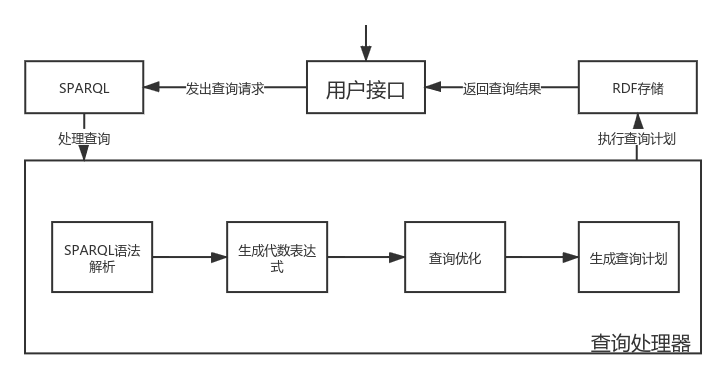
\includegraphics[width = 1\textwidth]{SPARQL}
\caption{SPARQL查询过程}
\label{SPARQL查询过程}
\end{figure}

\section{强化学习}[Reinforcement Learning]
\subsection{概述}[introduction]
强化学习(Reinforcement learning)\cite{RLIntroduction}是机器学习中的一个领域,这种方法主要思想是通过与环境的交互来学习。其来源于心理学中的行为主义理论,即有机体如何在环境给予的奖励或惩罚的刺激下,逐步形成对刺激的预期,产生能获得最大利益的习惯性行为。例如当婴儿开始学习走路时,他刚开始并不能掌握平衡,并不会直接学会走路,但他通过与周围环境的交互获得反馈,例如摔倒会给他带来疼痛感(惩罚),顺利走出第一步保持了平衡(奖励),婴儿就会知道每个动作的后果(获得惩罚或奖励),从而逐渐选择奖励最多的动作,直到完全学会走路(奖励最大化)。当我们从计算机科学的角度看待这种方法时,我们可以将其解释为一个函数。该函数尝试使奖励信号最大化,而无需告知必须采取何种行动。

很多形式的有监督机器学习方法通常都有很多的输入输出对,每一个输入输出都是提前备好的训练数据集,训练过程会被告知要采取哪些动作,但是强化学习不同于前者的是它必须通过尝试不同的动作,根据与环境的交互获得动作的反馈,从而确定采取哪些动作能产生最大的回报。强化学习更加专注于在线规划,需要在探索(在未知的领域)和遵从(现有知识)之间找到平衡。

\subsection{马尔科夫决策过程}[MDP]
从技术角度来看,强化学习是一种随机优化方法,它可以表述为马尔可夫决策过程(MDP)\cite{MDP}。其基本思想是,代理(agent)采取一系列行动,以优化MDP模型中的给定目标。
马尔科夫决策过程(MDP)是马尔科夫链(Markov Chains)的拓展,所以它需要满足马尔科夫链的属性。例如未来状态的进展仅取决于当前状态,而不取决于过去的状态和采取的动作。
一个马尔科夫决策过程可以形式化的表示为以下五元组:
\begin{equation}\label{MDP5}
\langle S, A, P(s,a),R(s,a),S_0 \rangle
\end{equation}
\begin{itemize}
    \item S代表Agent所有可能的状态。
    \item A代表Agent可以采取的所有动作来到达一下个状态。
    \item $S_{t+1}\sim P(s,a)$是在状态s通过采取动作a到达的新状态。
    \item $R(s,a)$代表在状态s通过采取动作a获得的奖励。
    \item $S_0$是在Agent初始时的状态。
\end{itemize}

总体的目标是找到一个决策策略$\pi :S\longmapsto A$(一个状态到动作的映射函数),使得期望的奖励最大化。
马尔科夫决策过程是一个从交互中学习的过程,\ref{Interaction}表示出了这个交互学习过程:Agent是学习者,它在某个状态下采取动作并且与环境交互,Agent从环境中获取到下一个状态和动作对应的奖励。状态信息通常需要编码,也被称为observations。
\begin{figure}[h]
    \centering
    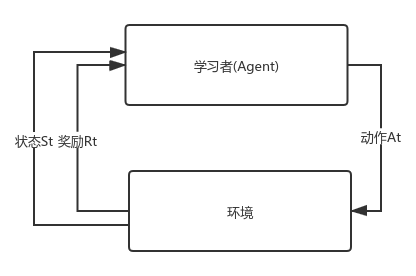
\includegraphics[width = 0.8\textwidth]{MDP}
    \caption{马尔科夫决策学习者与环境交互过程}
    \label{Interaction}
\end{figure}

\subsection{Q学习算法}
Q学习算法\cite{QLearning2}是由Watkins在其博士论文"Learning from delayed rewards"\cite{QLearning0}中第一次提出的,该算法是强化学习中具有里程碑意义的算法。Q学习算法是时间差分算法(TD)\cite{QLearning1}的一种,也是一种模型无关的算法,其主要针对具有折扣的奖励指标的控制。
 

% Local Variables:
% TeX-master: "../main"
% TeX-engine: xetex
% End:
